\documentclass[.../Dokumentation.tex]{subfiles}
\begin{document}
\subsection{Ergebnis}\label{sec-ita1-result}
Obwohl die in \ref{sec-ita1-cars} gezeigte Skizze die Dimensionen der zu 
installierenden Komponenten genau berücksichtigte, war der im Inneren des 
Fahrzeugs vorgesehene Platz nicht ausreichend bemessen.
Zu sehen ist diese Abweichung in Abbildung \ref{fig-car-too-small}.
Der Grund hierfür war, dass die Spezifikationen des gewählten Akkus nicht 
berücksichtigten, dass der Akku selbst zusätzlich in einer schützenden Hülle 
verpackt ist.\\
Um diese Hülle nicht entfernen zu müssen, wurde es also erforderlich, die 
Maße der Aussparung im Inneren des Fahrzeugs anzupassen. Dadurch ergab 
sich weiter der Bedarf diesen Zuwachs auch auf die Außenmaße anzuwenden.\\
\begin{figure}[H]
    \begin{center}
    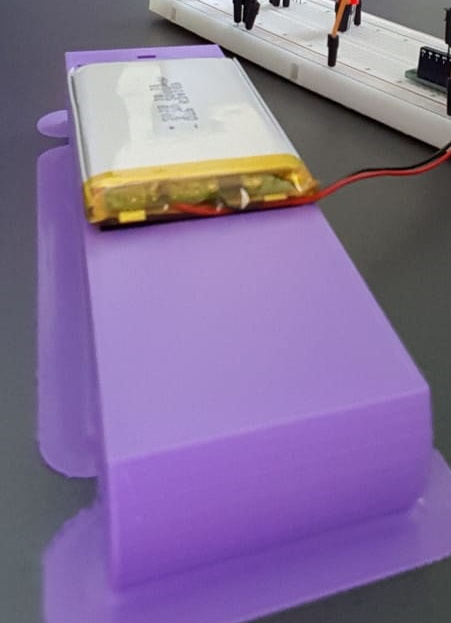
\includegraphics[
        width=0.5\linewidth,
    ]{imgs/car_too_small.jpg}
    \caption{Abweichende Maße des Akkus durch Hülle}
    \label{fig-car-too-small}
    \end{center}
\end{figure}
\noindent
Durch die Wahl einer abstrakteren Art der Darstellung für die anfallenden 
Emissionen hätte der persönliche Bezug zu diesen, durch die Bewegung der 
Fahrzeuge auf der in \ref{sec-concept} zur Sprache gekommenen Unterlage, seine 
Wirkung verlieren können. Obwohl also durch die Umsetzung mit Hall Sensoren 
eine recht präzise Messung der zurückgelegten Distanz möglich gewesen wäre, 
fiel an dieser Stelle die Entscheidung auf jedwede Art von Untergrund 
für die Fahrzeuge zu verzichten.
\end{document}